\documentclass{article}

% Language setting
% Replace `english' with e.g. `spanish' to change the document language
\usepackage[english]{babel}

% Set page size and margins
% Replace `letterpaper' with`a4paper' for UK/EU standard size
\usepackage[letterpaper,top=2cm,bottom=2cm,left=3cm,right=3cm,marginparwidth=1.75cm]{geometry}

% Useful packages
\usepackage{amsmath}
\usepackage{graphicx}
\usepackage[colorlinks=true, allcolors=blue]{hyperref}
\usepackage{float}
\usepackage{authblk}
\usepackage{caption}
\captionsetup[figure]{labelfont={bf},name={Figure},labelsep=period}
\captionsetup[table]{labelfont={bf},name={Table},position=top,labelsep=period}
\renewcommand{\thefigure}{S\arabic{figure}}
\setcounter{figure}{0}
\renewcommand{\thetable}{S\arabic{table}}
\setcounter{table}{0}

\title{Supporting Information: Electronic band structure screening for Dirac points in Heuslers}

\author{Meza-Morales, Paul J.} 
\author{Taliaronak, Volha} 
\author{Fumarola, Alessandro} 
\author{Shirsekar, Afrid} 
\author{kidner, Jonathan} 
\author{Ali, Zaheer}
\author{Ali. Mazhar}
\affil{Material Mind, Fremont, CA 94555, United States}
%\address{Material Mind, Fremont, CA 94555, United States}

%\author{Volha Taliaronak}
%\address{}
%\author{Alessandro Fumarola}
%\address{}
%\author{Afrid Shirsekar}
%\address{}
%\author{Jonathan kidner}
%\address{}
%\author{Mazhar Ali}
%\address{}

\begin{document}
\maketitle

%\begin{abstract}
%Your abstract.
%\end{abstract}
\section*{Section S1. Feature Engineering}
The table \ref{Tab:PF} lists properties used as primary features (PFs) and their definition. Tables \ref{Tab:PF_Cubic} and \ref{Tab:PF_Heusler} list the selected features for the development of Heusler and Cubic compounds datasets ML models respectively.

\begin{table}[H]
\caption{Primary features with their definitions}
\begin{tabular}{|l|l|}
\hline
\textbf{\begin{tabular}[c]{@{}l@{}}Electronic Property name/ \\ matminer abbreviation \end{tabular}}                             &   \textbf{Description/Matminer abbreviation} \\ \hline
\begin{tabular}[c]{@{}l@{}}maximum ionic charge/\\ max ionic char  \end{tabular}                        &   \begin{tabular}[c]{@{}l@{}}Element with the highest oxidation states in the crystal \\structure\end{tabular} \\ \hline
\begin{tabular}[c]{@{}l@{}}average ionic charge/\\ avg ionic char \end{tabular}                                &   \begin{tabular}[c]{@{}l@{}}Element with the highest oxidation states in the crystal \\structure \end{tabular} \\ \hline
\begin{tabular}[c]{@{}l@{}}ewald energy per atom/\\ewald\textunderscore energy\textunderscore per\textunderscore atom   \end{tabular}                         &   \begin{tabular}[c]{@{}l@{}}Computed energy from Coulombic interactions, using \\ charges already defined for the crystal structure\end{tabular} \\ \hline
\begin{tabular}[c]{@{}l@{}}HOMO element/\\ HOMO\textunderscore element \end{tabular}                                   &   \begin{tabular}[c]{@{}l@{}}Element with the highest occupied molecular orbital (HOMO) \\ estimated from the atomic orbital energies of the structure \\ chemical composition \end{tabular} \\ \hline
\begin{tabular}[c]{@{}l@{}}LUMO element/\\ LUMO\textunderscore element\end{tabular}                                   &  \begin{tabular}[c]{@{}l@{}}Element with the lowest unoccupied molecular orbital (LUMO) \\ estimated from the atomic orbital energies of the structure \\ chemical composition \end{tabular} \\ \hline
\begin{tabular}[c]{@{}l@{}}HOMO character/\\ HOMO\textunderscore character \end{tabular}                                 &   \begin{tabular}[c]{@{}l@{}}Atomic orbital character for the HOMO element \\ (`s', `p', `d', or `f') \end{tabular} \\ \hline
\begin{tabular}[c]{@{}l@{}}LUMO character/\\ LUMO\textunderscore character \end{tabular}                                 &  \begin{tabular}[c]{@{}l@{}}Atomic orbital character for the LUMO element \\ (`s', `p', `d', or `f') \end{tabular} \\ \hline
HOMO\textunderscore energy                                  &   \begin{tabular}[c]{@{}l@{}}Atomic orbital energy for the HOMO character \end{tabular} \\ \hline
LUMO\textunderscore energy                                  &  \begin{tabular}[c]{@{}l@{}}Atomic orbital energy for the LUMO character \end{tabular} \\ \hline
\begin{tabular}[c]{@{}l@{}} HOMO-LUMO atomic orbital gap/\\ gap\textunderscore AO  \end{tabular} &  \begin{tabular}[c]{@{}l@{}} bandgap from HOMO and LUMO energies \end{tabular} \\ \hline
\begin{tabular}[c]{@{}l@{}}fraction of s valence electrons/\\frac s valence electrons  \end{tabular}                     &    \begin{tabular}[c]{@{}l@{}}Weighted fraction of `s' valence electrons estimated from the \\ structure chemical composition \end{tabular} \\ \hline
\begin{tabular}[c]{@{}l@{}}fraction of p valence electrons/\\frac p valence electrons \end{tabular}                      &    \begin{tabular}[c]{@{}l@{}}Weighted fraction of `p' valence electrons estimated from the \\ structure chemical composition \end{tabular} \\ \hline
\begin{tabular}[c]{@{}l@{}}fraction of d valence electrons/\\frac d valence electrons  \end{tabular}                     &    \begin{tabular}[c]{@{}l@{}}Weighted fraction of `d' valence electrons estimated from the \\ structure chemical composition \end{tabular} \\ \hline
\begin{tabular}[c]{@{}l@{}}fraction of f valence electrons/\\frac f valence electrons  \end{tabular}                     &    \begin{tabular}[c]{@{}l@{}}Weighted fraction of `f' valence electrons estimated from the \\ structure chemical composition \end{tabular} \\ \hline
%\textbf{Size}                                    &   \textbf{Description} \\ \hline
%Covalent Radius                                 &   \\ \hline
\textbf{Crystal}                                &   \textbf{Description} \\ \hline
Density                                         &   Crystal density \\ \hline
Volume per atom                                 &   \begin{tabular}[c]{@{}l@{}}Average volume taken up by an atom in the crystal \\ structure\end{tabular} \\ \hline
structural complexity per cell                  &   \begin{tabular}[c]{@{}l@{}}Shannon information entropy of a structure. This \\descriptor treat a structure as a message to evaluate \\structural complexity (bits/cell)\end{tabular} \\ \hline
structural complexity per atom                  & \begin{tabular}[c]{@{}l@{}}Shannon information entropy of a structure. This \\descriptor treat a structure as a message to evaluate \\structural complexity (bits/atom)\end{tabular} \\ \hline
max packing efficiency                          &   \begin{tabular}[c]{@{}l@{}}Maximum possible packing efficiency of this structure\end{tabular} \\ \hline
mean neighbor distance variation                &   \begin{tabular}[c]{@{}l@{}}Statistic (e.g., mean) of the neighbor distance variation\end{tabular} \\ \hline
mean absolute deviation in relative cell size   &   \begin{tabular}[c]{@{}l@{}}Voronoi cell volume across all sites in the structure, \\divided by the mean Voronoi cell volume\end{tabular} \\ \hline
mean absolute deviation in relative bond length & \begin{tabular}[c]{@{}l@{}}The average bond lengths for all sites, divided by the \\average bond length\end{tabular} \\ \hline
%\textbf{Bulk}                                   &   \textbf{Description} \\ \hline
%density                                         &   Crystal density\\ \hline
%Melting Point                                   &   \\ \hline
\end{tabular}
\label{Tab:PF}
\end{table}

\begin{table}[H]
\caption{Heusler dataset ML model features}
\begin{tabular}{|l|}
\hline
\textbf{Electronic}                             \\ \hline
frac s valence electrons                        \\ \hline
frac d valence electrons                        \\ \hline
max ionic char                                  \\ \hline
HOMO\textunderscore element                                    \\ \hline
avg ionic char                                  \\ \hline
gap\textunderscore AO                                          \\ \hline
LUMO\textunderscore element                                    \\ \hline
LUMO\textunderscore energy                                     \\ \hline
HOMO\textunderscore character                                  \\ \hline
LUMO\textunderscore character                                  \\ \hline
frac f valence electrons                        \\ \hline
frac p valence electrons                        \\ \hline
HOMO\textunderscore energy                                     \\ \hline
ewald\textunderscore energy\textunderscore per\textunderscore atom  \\ \hline
\textbf{Crystal}                                \\ \hline
structural complexity per atom                  \\ \hline
mean absolute deviation in relative cell size   \\ \hline
structural complexity per cell                  \\ \hline
mean neighbor distance variation                \\ \hline
mean absolute deviation in relative bond length \\ \hline
volume per atom                                 \\ \hline                   
packing fraction                                \\ \hline
max packing efficiency                          \\ \hline
density                                         \\ \hline
%\textbf{Bulk}                                   \\ \hline
%density                                         \\ \hline
%Melting Point                                   \\ \hline
\end{tabular}
\label{Tab:PF_Heusler}
\end{table}

\begin{table}[H]
\caption{Cubic dataset ML model features}
\begin{tabular}{|l|}
\hline
\textbf{Electronic}                            \\ \hline
HOMO\textunderscore element                                   \\ \hline
LUMO\textunderscore character                                 \\ \hline
LUMO\textunderscore element                                   \\ \hline
frac d valence electrons                       \\ \hline
max ionic char                                 \\ \hline
LUMO\textunderscore energy                                    \\ \hline
HOMO\textunderscore energy                                    \\ \hline
frac s valence electrons                       \\ \hline
frac p valence electrons                       \\ \hline
packing fraction                               \\ \hline
frac f valence electrons                       \\ \hline
ewald\textunderscore energy\textunderscore per\textunderscore atom      \\ \hline
avg ionic char                                 \\ \hline
HOMO\textunderscore character                                 \\ \hline
gap\textunderscore AO                                         \\ \hline
\textbf{Crystal}                               \\ \hline
structural complexity per cell                 \\ \hline
structural complexity per atom                 \\ \hline
max packing efficiency                         \\ \hline
mean neighbor distance variation               \\ \hline
volume per atom (vpa)                               \\ \hline
mean absolute deviation in relative cell size  \\ \hline
mean absolute deviation in relative bond length \\ \hline
density                                         \\ \hline
%\textbf{Bulk}                                   \\ \hline
%density                                         \\ \hline
%Melting Point                                   \\ \hline
\end{tabular}
\label{Tab:PF_Cubic}
\end{table}

%\section*{Section S2. ML Models: Principal Component Analysis (PCA) features}

\section*{Section S2. Band Structure Features Detection}
\begin{figure}[H]
    \centering
    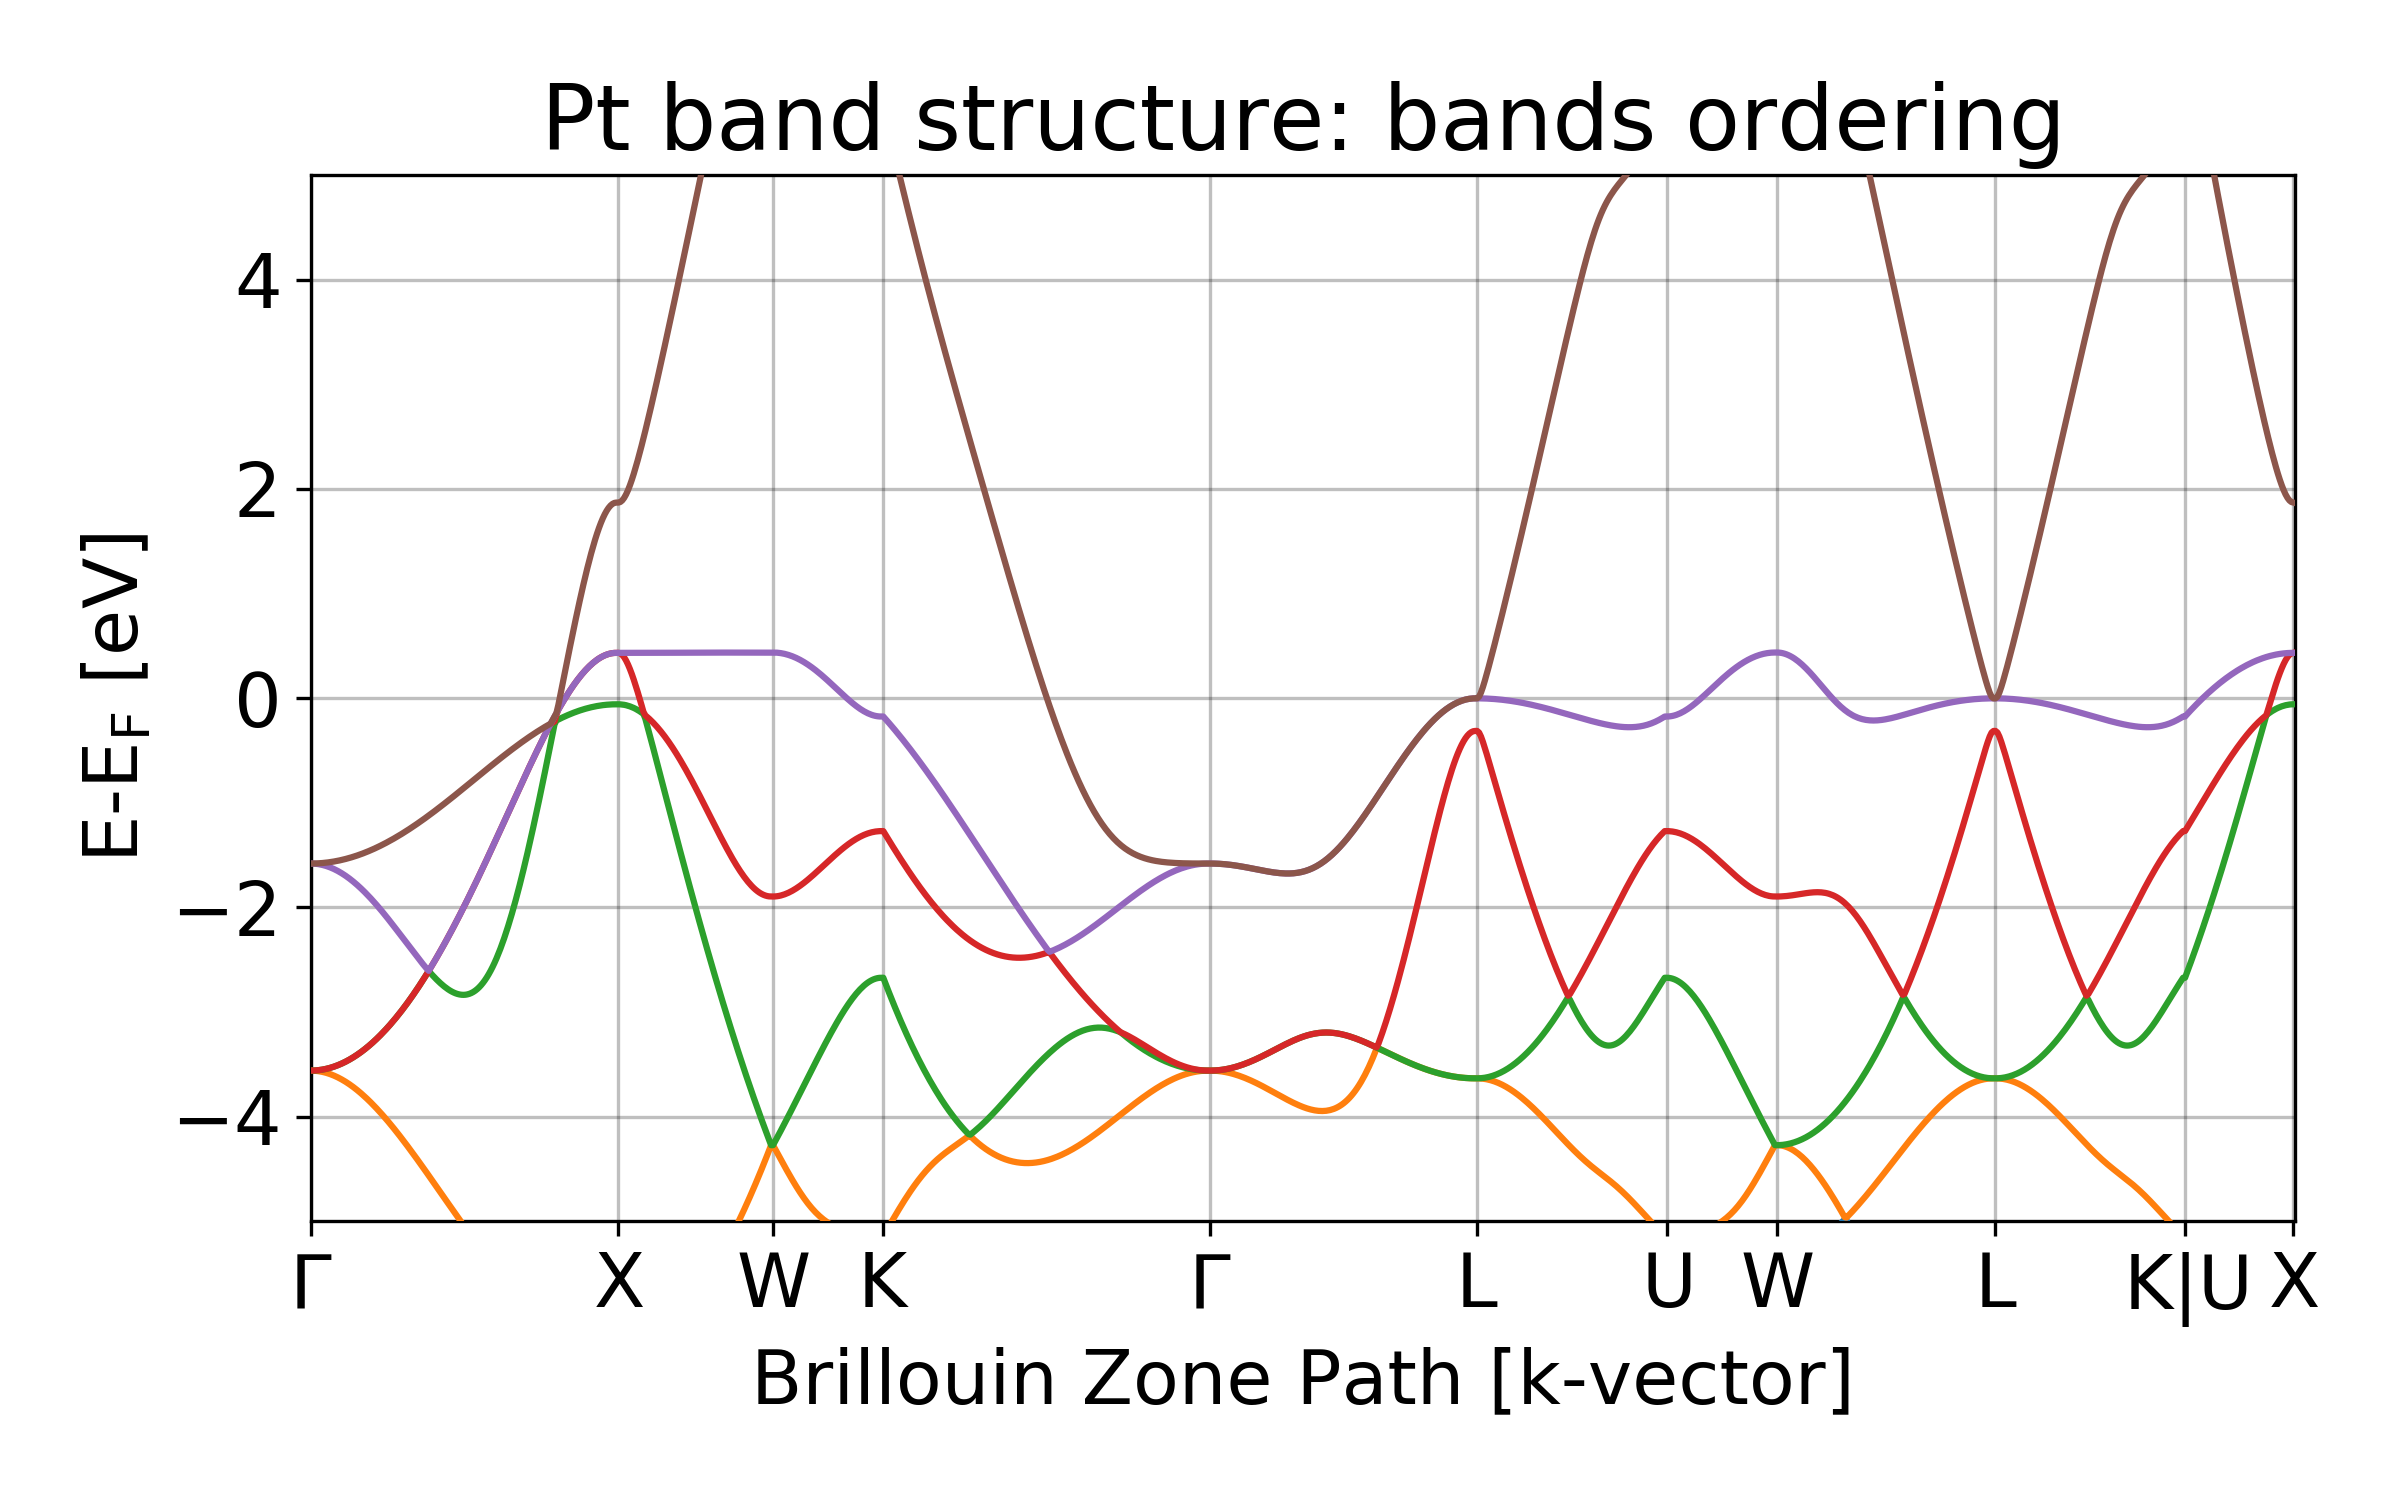
\includegraphics[width=0.75\textwidth]{SI/figures/mp-126_band-structure_order.png}
    \caption{pymatgen band structure of cubic elemental Platinum (Pt, space group 225, \href{https://materialsproject.org/materials/mp-126/}{mp-126 on Materials Project}). Each individual band is plotted in a different color. The relative order of the bands does not change across the BZ path. The band plotted in brown is the highest in the y-axis range, while the orange one is the lowest.}
    \label{fig:bands_order}
\end{figure}

Automatic detection and identification of band structure features can dramatically accelerate large-scale discovery of materials property. The number and type of band structure features are detected using an algorithm developed in \textit{python} with the numerical library \textit{numpy} as the only functional dependency (other libraries are needed for visualization, data management and debug).

The input data is a \href{https://materialsproject.org/materials/mp-126/}{\texttt{pymatgen.electronic\_structure.bandstructure.BandStructure}} object with the bands represented as a $M \cdot N$ \texttt{numpy.array} of eigenvalues. $M$ is the number of bands calculated for the given material while $N$ is the number of reciprocal space locations sampled for each band. A separate array \texttt{BandStructure.kpoints} of shape $N \cdot 3$ is also provided to locate the k-points within the Brillouin Zone. The sequence of k-points follows the Setyawan-Curtarolo \cite{setyawan2010high} convention.

Band structure features usually arise from the interaction of multiple bands. The first step of the feature detection algorithm consists in producing the band indexes $i,j \in [1,M]$ of the bands that need to be compared. All three types of features we are focusing on (i.e. degeneracy lines, degeneracy points and gaps) are characteristic of the interaction between two bands, but there is no theoretical limitation to the number of bands that contributes to the calculation. Bands in \textit{pymatgen} keep their relative order which means that if a band has a largest energy value at the $\Gamma$ point with respect to another, it will keep a higher or equal value for the whole Brillouin Zone path. For this reason, we never compare bands whose indexes are too far from each other as they will most likely have a large energy difference and small interaction. Each band is compared with the 2 closest higher bands and the 2 lower.

\begin{verbatim}
    def find_degeneracy_lines(
        eigenvalues,        # M x N matrix with band structure
        max_delta_energy,   # maximum energy difference
                            # for degenerate bands
        delta_k,            # minimum number of consecutive
                            # degenerate points to form a degenerate line
                            )
        # Calculate indexes of the bands that need to be
        # combined
        index_a, index_b = make_combinations(
                                eigenvalues.shape[0],
                                n_bands_in_combination = 2
                                )
                                
        band_a = eigenvalues[index_a,:] # Shape 1 x N
        band_b = eigenvalues[index_b,:] # Shape 1 x N
        diffs = band_b - band_a         # Shape 1 x N
        
        # Sequence of Boolean operations to verify
        # existence of a band structure feature
        condition = (diffs<=max_delta_energy)   # Shape 1 x N
        
        # If a sequence of true values is shorter
        # than delta_k, set all the sequence to False
        condition = filter_short_sequences(
                        condition,
                        delta_k
                        )
        
        k_indexes = where(condition == True)
        
        return k_indexes
        
\end{verbatim}

The band pairs are sequentially inputted to the function  \texttt{find\_feature()} together with auxiliary parameters which determine the type of feature the user wants to detect. For each run of the \texttt{find\_feature()} function, that is the detection of a given feature, we assign a truth value to each eigenvalue of the band pairs. If at the end of the function this value is \texttt{True}, it means that the desired feature is found at the assigned array index $k < N$ (each index corresponds to a reciprocal space location). A series of binary checks are performed on the band values and their combination to determine whether the conditions apply to detect a feature. A pseudo-code to detect degeneracy lines is reported above.

\begin{figure}[H]
    \centering
    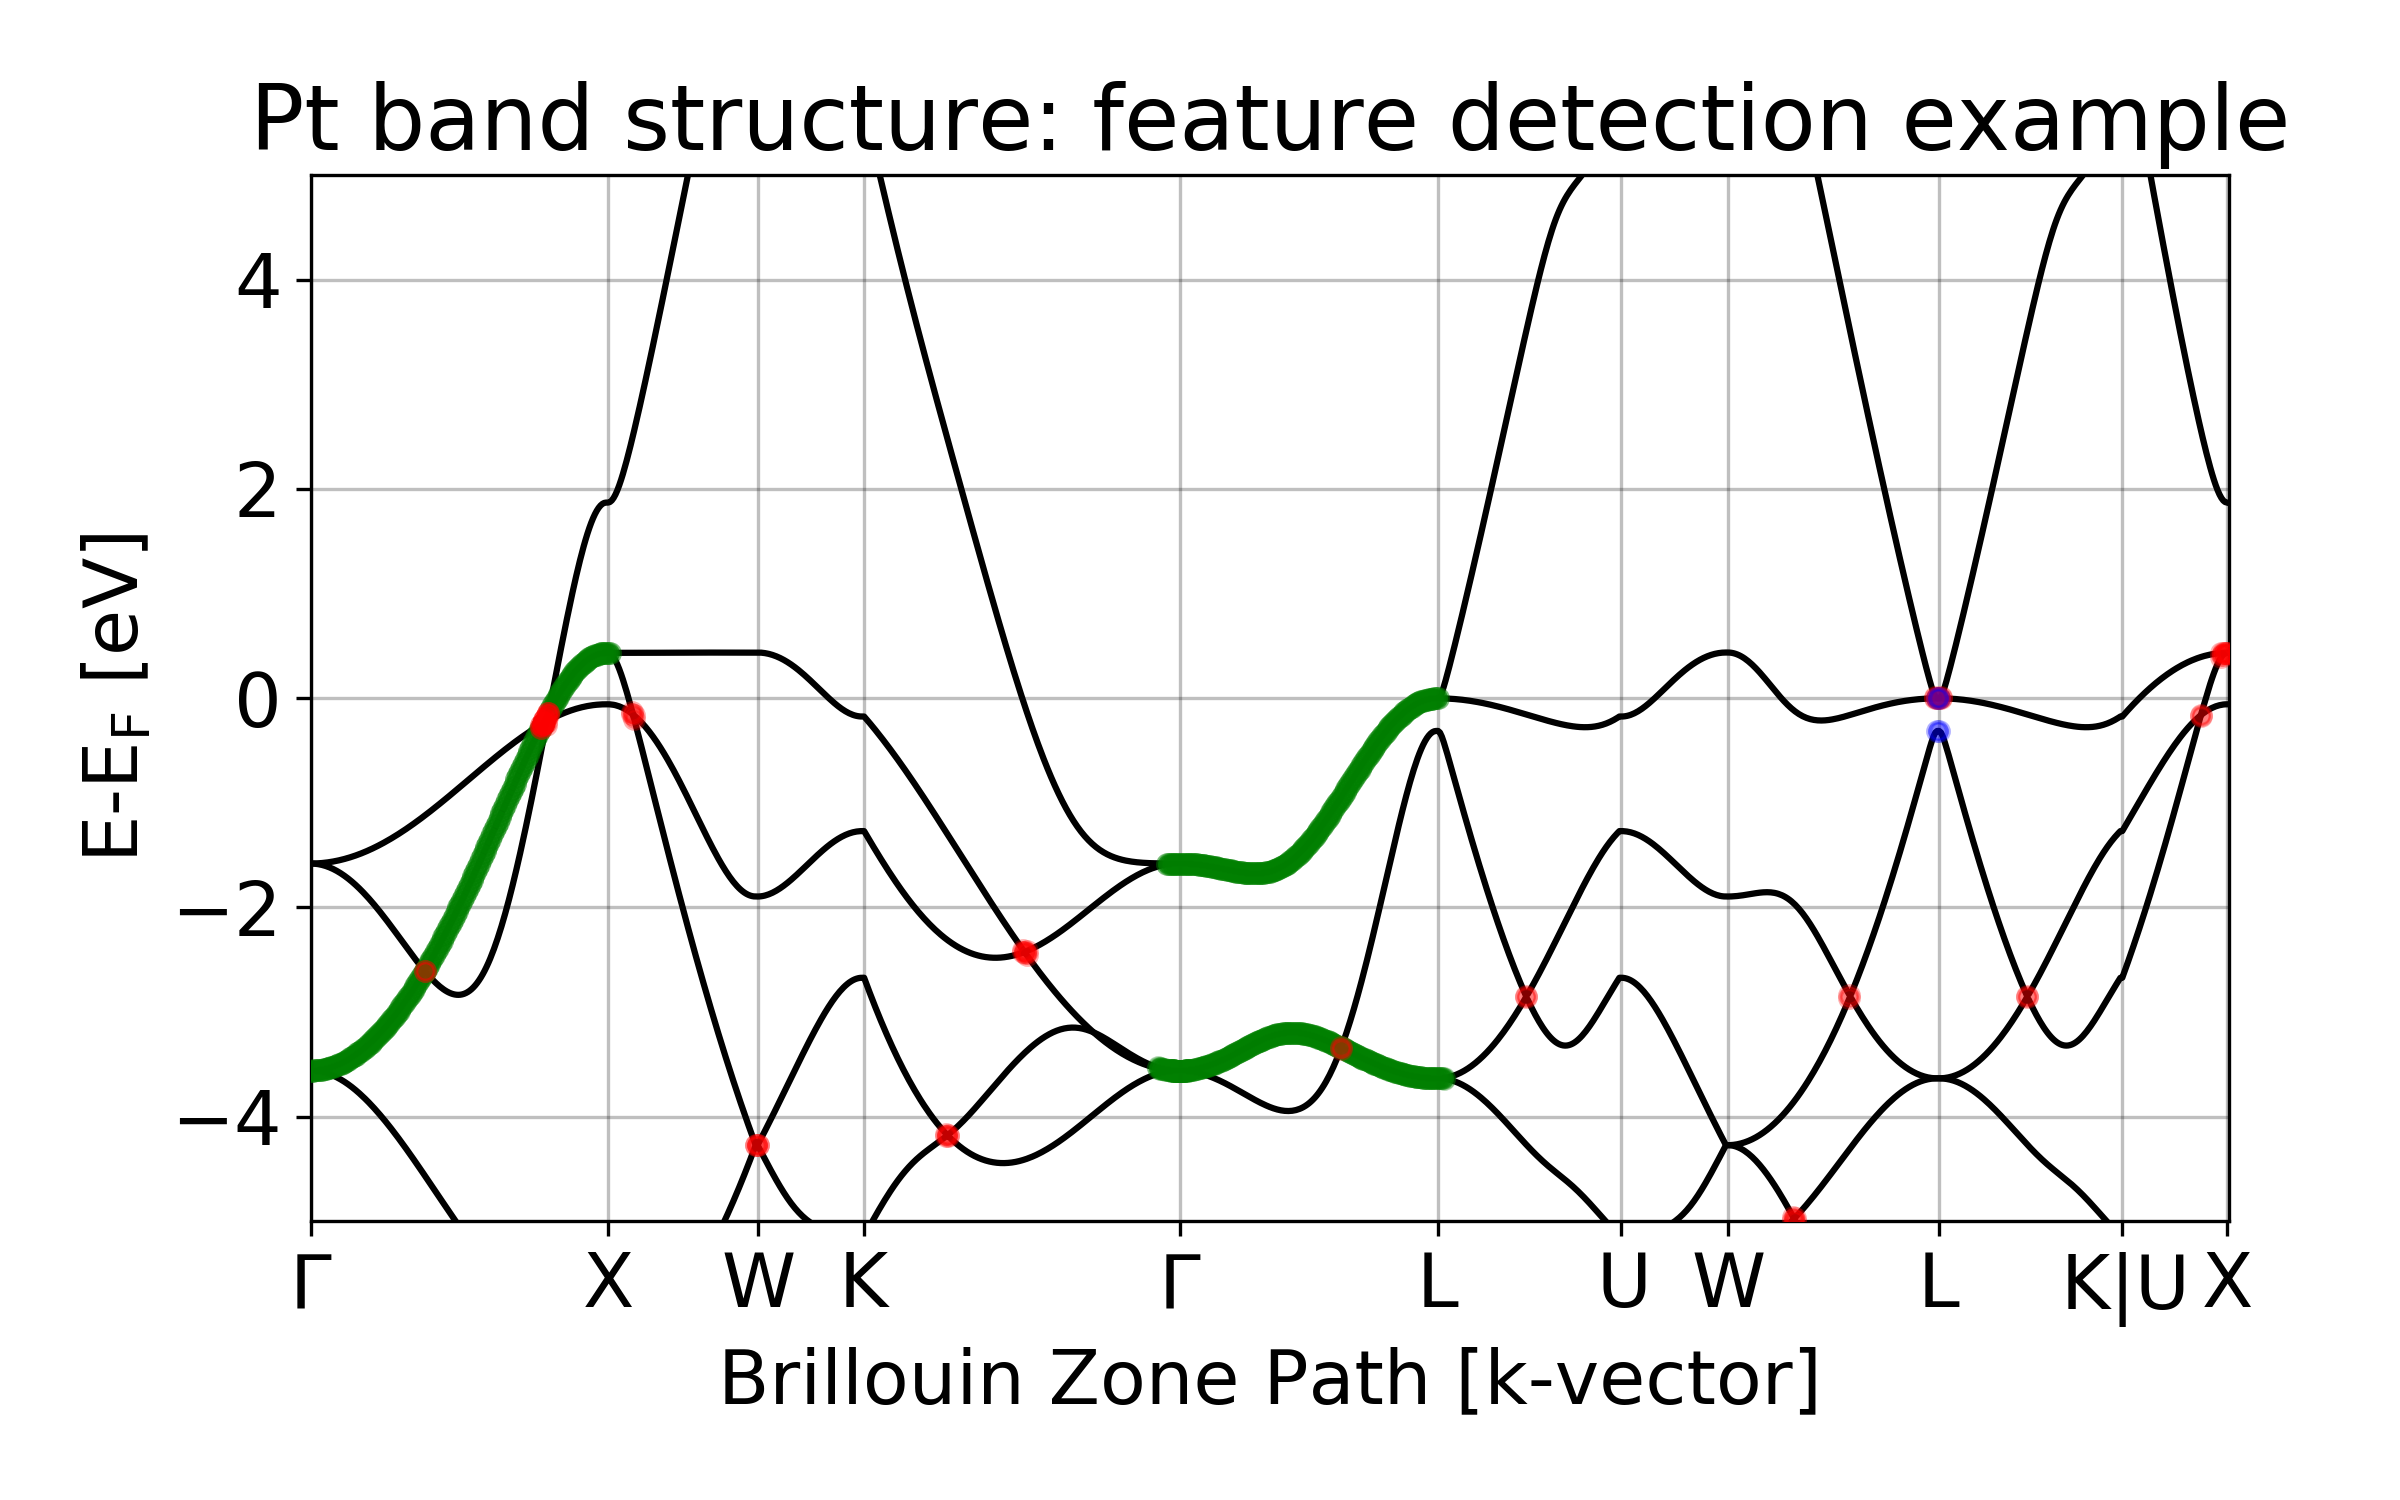
\includegraphics[width=0.75\textwidth]{SI/figures/mp-126_band-structure_features.png}
    \caption{Band structure of cubic elemental Platinum (Pt, space group 225, \href{https://materialsproject.org/materials/mp-126/}{mp-126 on Materials Project}). The eigenvalues are plotted in black, the degeneracy lines are highlighted in green. The degeneracy points and inter-band gaps are highlighted in red and blue respectively}
    \label{fig:feature_detection}
\end{figure}

%\bibliographystyle{alpha}
%\bibliography{sample}

\end{document}